\documentclass{article}
\usepackage[utf8]{inputenc}
\usepackage[margin=1in]{geometry}
\usepackage{parskip}
\usepackage{alltt}
\usepackage{amsmath}
\usepackage{fixltx2e}
\usepackage{hyperref}
\usepackage{graphicx}


\begin{document}
\begin{flushright}
Samson Shi.354

\today

CSE 3461 Homework 2
\end{flushright}

\begin{enumerate}

\item[1]\textbf{(6 points)} UDP and TCP use one’s complement for their checksums. Suppose we have the following 8-bit bytes: \texttt{01010011, 01100110, 01110100}. (While UDP and TCP use 16-bit words to compute the checksum, this problem only concerns 8-bit bytes.) Answer the following questions:

\begin{enumerate}
  \item \textbf{(2 points)} What is the one’s complement of the sum of these bytes? Show all your work.

  \texttt{01010011} + \texttt{01100110} = \texttt{10111001}

  \texttt{10111001} + \texttt{01110100} = \texttt{00101110}

  Checksum is found by taking the 1's complement of the solution, so the checksum = \texttt{11010001}

  \item \textbf{(2 points)} Why does UDP use the one’s complement of the sum, not the sum?

  UDP uses the 1's complement of the sum to allow for quick error detection. On the receiver side, all four words are added together, including the checksum. This results in a sum of all 1's if there are no errors.

  \item \textbf{(2 points)} How does the receiver detect errors? Can 1-bit or 2-bit errors go undetected? Explain your answer.

  Error detection is done by summing all four numbers as detailed in part (b). Any 0's that exist in the sum are easily detected. 

\end{enumerate}

\item[2]\textbf{(6 points)} Consider the Go-Back-N (GBN) protocol with a sender window size of $w$ and a sequence number range of $sn$. Suppose that at time $t$, the next in-order packet that the receiver is expecting has a sequence number of $k$. Assume messages are not reordered. Answer the following questions (and justify your answers):

  \begin{enumerate}
  \item \textbf{(3 points)} What are the possible sets of sequence numbers inside the sender’s window at time $t$?

  One possible set of sequence numbers would be if the $k-1$ sequence was just sent and ACK's were received by the sender, resulting in the window $(k, k + w - 1)$. The other set of sequence numbers would be if none of the messages were ACK'd, resulting in $(k - w, k - 1)$.

  \item \textbf{(3 points)} What are all possible values of the ACK fields in all possible messages currently propagating back to the sender at time $t$?

  If the receiver is waiting for packet $k$, then all previous packets must have been received and ACK'd. Otherwise, if none of the ACK's were received by the sender, then it could still be propogating. However, since the $k$th packet had been sent out, the sender must have recieved the packets before. Thus, the possible values of the ACK fields in all possible messages could range from $k - w - 1$ to $k - 1$. 

  \end{enumerate}
 
\item[3]\textbf{(6 points)} Consider the GBN and SR protocols. Suppose the sequence number space has size $k$. What is the largest allowable sender window that will avoid the occurrence of problems such as that in Figure 3.27 for each protocol?

For GBN, the largest allowable sender window that will avoid the occurrence of problems seen in Figure 3.27 is any size since GBN can discard out of order packets.

For SR, the largest allowable sender window that will avoid the occurrence of problems seen in Figure 3.27 is of size $k/2$.

\item[4]\textbf{(4 points)} Describe the purpose of shortcuts in a DHT with an example.

The purpose of shortcuts is to find a good balance between connecting all peers to each other and a normal circular DHT. Having each peer be aware of all $N-1$ peers is not a very elegant solution, and having each peer only aware of the two surrounding peers gives an average of $N/2$ lookups per query, which is also not desirable. Shortcuts connect each peer to a handful of other nodes which results in the ability for the node to query a neighboring node that is closer to the key.

An example of shortcuts with DHT is if a node at position 3 wants to know who is responsible for key 11. In a circular DHT, node 3 would query 4, and then 5, and then 8, then 10, and finally to 12. With shortcuts, 3 instead can query 8 instantly because of the shortcut and then 8 can go to 10 and then 12. 

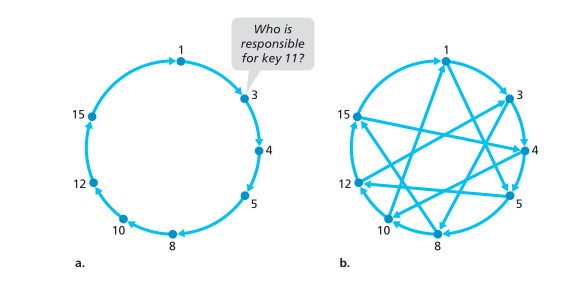
\includegraphics{DHT.png}
    
\item[5]\textbf{(4 points)}Define the terms $torrent$, $seed$, and $leecher$ in the context of BitTorrent. (You may need to search outside the book for some of these terms).

Torrent: A torrent file is a type of file that includes metadata about the files and folders for data that is to be downloaded over a BitTorrent p2p connection. It also usually includes network locations for trackers. The torrent file itself does not actually include any of the data that is to be downloaded but rather information about the files, like names, sizes, folder structure, and hash values which can be used to verify file integrity.

Seed: A seed is a person that has a torrent file open in their torrent client of choice and has the whole file downloaded and are actively uploading the file (seeding) to their peers but are not downloading.

Leecher: A leecher is a personthat does not have the file donloaded yet and are not just uploading the file to other peers.


\item[6]\textbf{(6 points)} ) Consider transferring an enormous file of $L$ bytes from Host A to Host B. Assume an MSS of 536 bytes.

  \begin{enumerate}
  \item \textbf{(3 points)} What is the maximum value of L such that TCP sequence numbers are not exhausted? Recall that the TCP sequence number field has 4 bytes.

  If a TCP sequence number has 4 bytes, the maximum value of a sequence number is $2^{32} = 4,294,967,296$. 

  Thus, if the maximum sequence size is 536 bytes, the maximum size of $L$ would be $MSS * 4,294,967,296 = 2,302,102,470,656 bytes$

  \item \textbf{(3 points)} For the $L$ you obtain in (a), find how long file transmission takes. Assume that a total of 66 bytes of transport, network, and data-link header are added to each segment before the resulting packet is sent out over a 155 Mbps link. Ignore flow control and congestion control so A can send the segments back-to-back and continuously.

  $4,294,967,296 segments * 66 bytes + 2,302,102,470,656 bytes =  2,585,570,312,192 bytes$

  $2,585,570,312,192 bytes / 155 Mbps = 2,585,570,312,192 bytes / 155,000,000 Bytes/Sec = 16,681 seconds$

  \end{enumerate}

\item[7]\textbf{(8 points)} ) ) Read the man pages for \texttt{netstat} and \texttt{ping} to answer the following questions.

  \begin{enumerate}
  \item \textbf{(6 points)} Explain the options \texttt{-a} and \texttt{-p} for \texttt{netstat}. Start an FTP connection using the command \texttt{ftp <ftp-site-address>}. You can pick any FTP site. A few publicly available FTP sites are listed at \texttt{http://www.gnu.org/prep/ftp.html}. After you login as anonymous, try to find information regarding the corresponding TCP connection using netstat in a different window. Explain the fields in the line corresponding to your ftp connection. What are the local and remote port numbers and IP addresses for that TCP connection? You do not need to submit the complete output of netstat, but you need to submit a printout of the line corresponding to your FTP connection. (Hint: What is the dedicated port used by FTP?)

  -a: Shows both listening and non listening sockets

  -p: Shows the PID and name of the program to which each socket belongs

  I used \texttt{netstat -tan | grep \:21} to find information on the addresses in numerical form as well as to grab only entries that contained port number 21, which is the default port for FTP.

  Local Address: 192.168.1.129:53648

  Remote Address: 199.204.44.194:21

  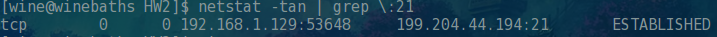
\includegraphics[scale=0.5]{netstat.PNG}

  \item \textbf{(2 points)} Try out the following options with \texttt{ping: -s} and \texttt{-i}. Explain the outputs. For this question, you don’t have to submit the output of \texttt{ping}.

  -s: sets the size of the packet that the user sends in a ping. Default size is 56 bytes.

  -i: sets the time interval between packets sent. Default is 1 second, requires sudo access for anything less than .2 seconds


  \end{enumerate}
\end{enumerate}

\end{document}